\documentclass{article}
\usepackage[utf8]{inputenc}
\usepackage{graphicx}
\usepackage{amsmath }
\usepackage{amssymb}
\usepackage{subcaption}
\usepackage{float}
\setcounter{section}{1}


\usepackage{cleveref} %referencing figures, equations and tables
\crefformat{figure}{Figure.~#2#1#3}
\crefformat{equation}{Eq.~#2#1#3}
\crefformat{table}{Table.~#2#1#3}
\crefformat{appendix}{Appendix.~#2#1#3}
\crefformat{section}{Section.~#2#1#3}

\title{Wave Propagation in a Cantilever Beam Under Normal Load}
\author{Amir Baharvand }
\date{}

\begin{document}

\maketitle

\subsection{Applied Load in Form of the Dirac Delta Function}

The problem description is provided in \cite{ACHENBACH:1975} (problem 8.1) with the step function. In the present problem, the step function is replaced by Dirac Delta function.

\subsection{Problem Statement}
The one-dimensional wave equation can be expressed in the form of

\begin{equation}
    \dfrac{\partial^2 u}{\partial t^2} = c^2 \dfrac{\partial^2 u}{\partial x^2}
    \label{eq:wave_eqn}
\end{equation}

where $x$ and $t$ denote position and time. $u$ is the displacement and is a function of both $x$ and $t$ and $c$ is the velocity of wave propagation. For the problem under study, which is the wave propagation in a cantilever beam under normal stress, the initial and boundary conditions (I.C and B.C) are defined as below.

\begin{equation*}
\begin{matrix}
    \text{I.C}\begin{cases}
        u(x, 0) = 0 \\ 
        \\
        \dfrac{\partial u(x, 0)}{\partial t} = 0 
    \end{cases} \quad , \quad
    \text{B.C}\begin{cases}
        u(0, t) = 0 \\
        \\
        \dfrac{\partial u(L, t)}{\partial x} = \dfrac{P(t)}{EA}
    \end{cases}
\end{matrix}
\end{equation*}

In the above equations, $L$ is the length, $P(t)$ is the applied force at the right end of the beam, $E$ is the Young's modulus and $A$ is the cross-sectional area of the beam (\cref{fig:beam}).

\begin{figure}[H]
    \centering
    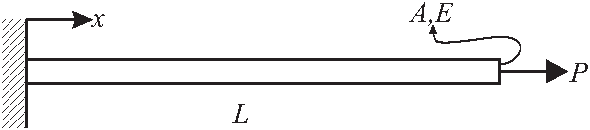
\includegraphics[width = 0.6\textwidth ]{figures/beam.pdf}
    \caption{Cantilever beam geometry, boundary condition and coordinate system.}
    \label{fig:beam}
\end{figure}

\section{Applied Load in Form of the Step Function}

In this section, the step function is replaced by the Dirac delta function, $\delta(t)$, that is $P(t) = P \delta(t)$ only exist at $t = 0$. The solution for this part is performed by Maple. However, one may use the Laplace inverse approach from \cite{Spiegel1965} similar to the previous section.

\begin{equation}
    \mathcal{L}^{-1}\{ \frac{\sinh(sx)}{s \cosh(sL)} \} = \frac{4}{\pi} \sum_{n = 1}^{\infty} \frac{(-1)^n}{(2n - 1)} \sin \left( \frac{(2n-1)\pi}{2L}x\right) \sin \left( \frac{(2n-1)\pi}{2L}t\right)
    \label{eq:d_lap_inv}
\end{equation}

Normalized longitudinal displacement and stress for this case of loading are shown in \cref{fig:u_sigma_dirac}. The displacement has a constant value as the generated tensile wave travels to the fixed boundary on the left and bounces back as another tensile wave until it reaches the right side. The whole process takes $t = 2$s. As the applied load is now absent, the right side of the beam acts as a free boundary and the wave reflects as a compressive which is evident in \cref{fig:u_sigma_dirac}(a) by changing the displacement sign. The periodicity for this procedure is $t = 4$s. Due to the constant displacement, the stress becomes zero ($\sigma_x = \rho c \dfrac{\partial u}{\partial x}$ where $\rho$ is density.).


\begin{figure}[H]
        \begin{subfigure}{1\textwidth}
            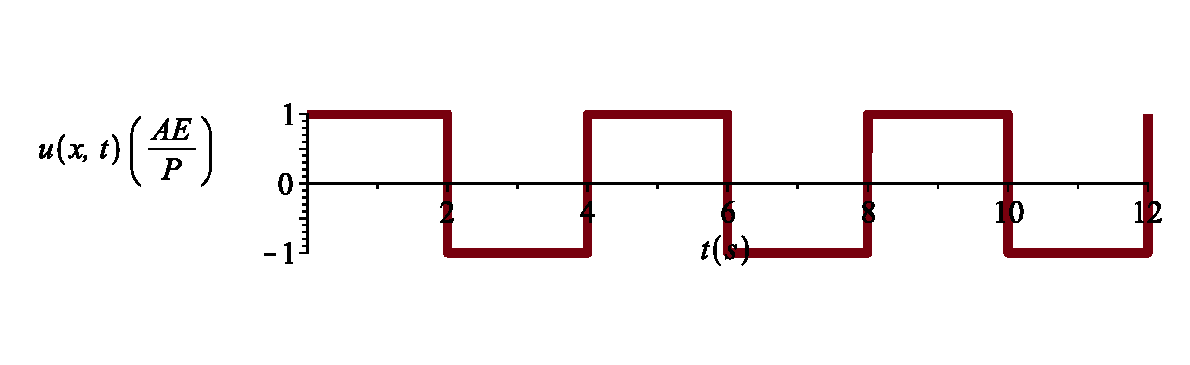
\includegraphics[width=0.9\columnwidth]{figures/d_u.eps} 
            \caption{}
            % \label{}
        \end{subfigure}
        \begin{subfigure}{1\textwidth}
            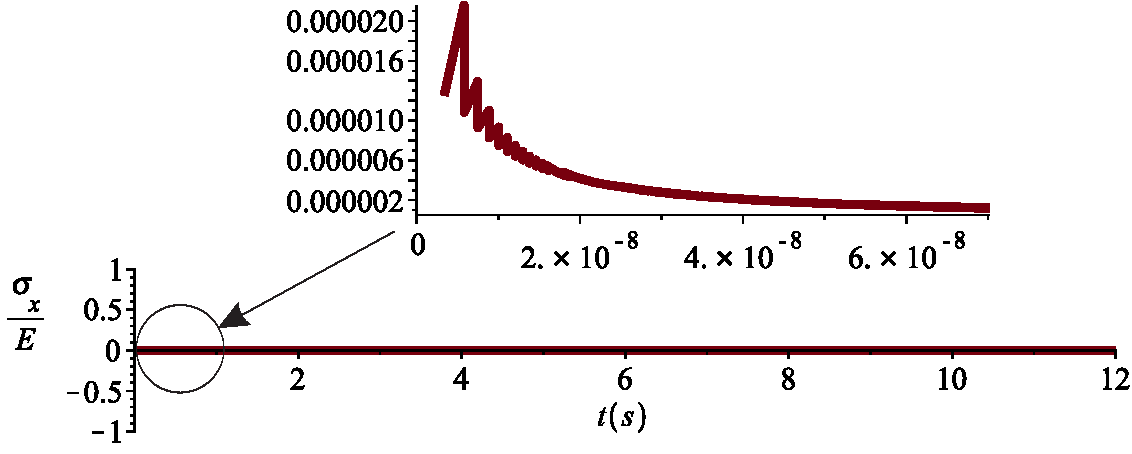
\includegraphics[width=0.9\columnwidth]{figures/d_sigma.pdf} 
            \caption{}
            % \label{}
        \end{subfigure}
    \caption{Case $P \delta(t)$: Normalized (a) longitudinal displacement, $u(x, t)$ and (b) stress, $\sigma_x$ for different time increments ($L$, $c$ and $x$ equal to 1) for the case $P(t) = P \delta(t)$. Number of terms in the series is 1000.}
    \label{fig:u_sigma_dirac}
\end{figure}


\newpage
\bibliography{ref}
\bibliographystyle{ieeetr}

\end{document}